\section{Présentation et caractéristiques des machines}\label{sec:contribs:machines}

Nous présentons dans cette sections deux machines NUMA de générations différentes et au caractéristiques assez différentes.
La première, \emph{idchire}, est basée sur des processeurs Intel Sandy Bridge, et possède un nombre important de nœuds NUMA.
La seconde, \emph{brunch}, est basé sur des processeurs Intel plus récents de la génération Broadwell, et dispose d'un nombre assez faible de nœud NUMA.

\subsection{idchire}\label{sec:contribs:machines:idchire}


Cette machine est équipée de 24 processeurs Intel(R) Xeon(R) CPU E5-4640 (Sandy Bridge), cadencés à 2.4 GHz.
Chacun de ce processeurs est associé à 31 Go de RAM pour former un nœud NUMA, ils disposent de 8 cœurs physiques partageant 20 Mo de cache L3 (20-ways associatif).
Chacun des cœur à accès à 32 Ko de cache L1 (données) et 256 Ko de cache L2 (8-ways associatif).
Les latences et bandes passantes relatives à chacun des niveaux de cache sont présentées dans le tableau~\ref{tab:synthese-processeurs}.

La machine entière dispose donc de 192 cœurs physiques, et de 744 Go de RAM.
Les processeurs Sandy Bridge disposent de l'extension vectorielle AVX, permettant d'effectuer 4 additions et 4 multiplication de nombres flottant à double précision en un cycle, portant le pic de performance théorique de la machine à 3.6 TFLOPs.

\subsubsection{Topologie}

\begin{figure}[ht]
  \centering
  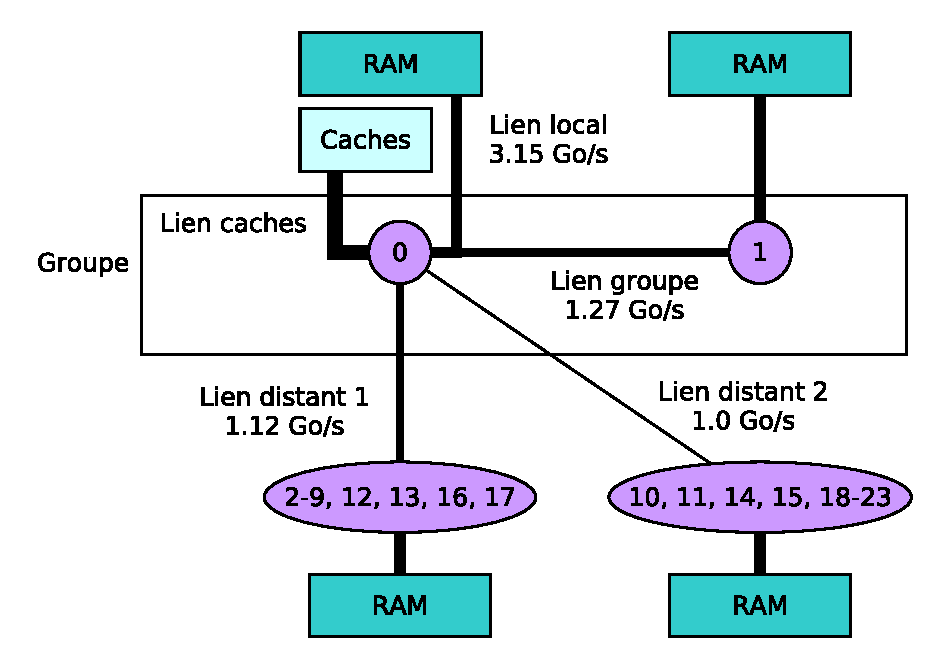
\includegraphics[width=0.8\textwidth]{topo-idchire}
  \caption{Topologie schématique vu du nœud 0}\label{fig:contribs:machines:idchire:topo-liens}
\end{figure}

L'interconnexion des nœuds NUMA est effectué à travers l'Intel \emph{Quick Path Interconnect} (QPI).
La topologie de la machine expose une hiérarchie à plusieurs niveaux, la Figure~\ref{fig:contribs:machines:idchire:topo-liens} présente la hiérarchie de la machine du point de vue du nœud 0.
Chaque nœud est d'abord associé à un autre nœud pour former un groupe. Ces groupes sont ensuite interconnectés entre eux et sont accessibles en deux rebonds maximum dans le système d'interconnexion.
Pour chaque nœud il y a 12 nœuds situés à un rebond, et 10 nœuds situés à deux rebonds.

\begin{figure}[t!]
  \centering
  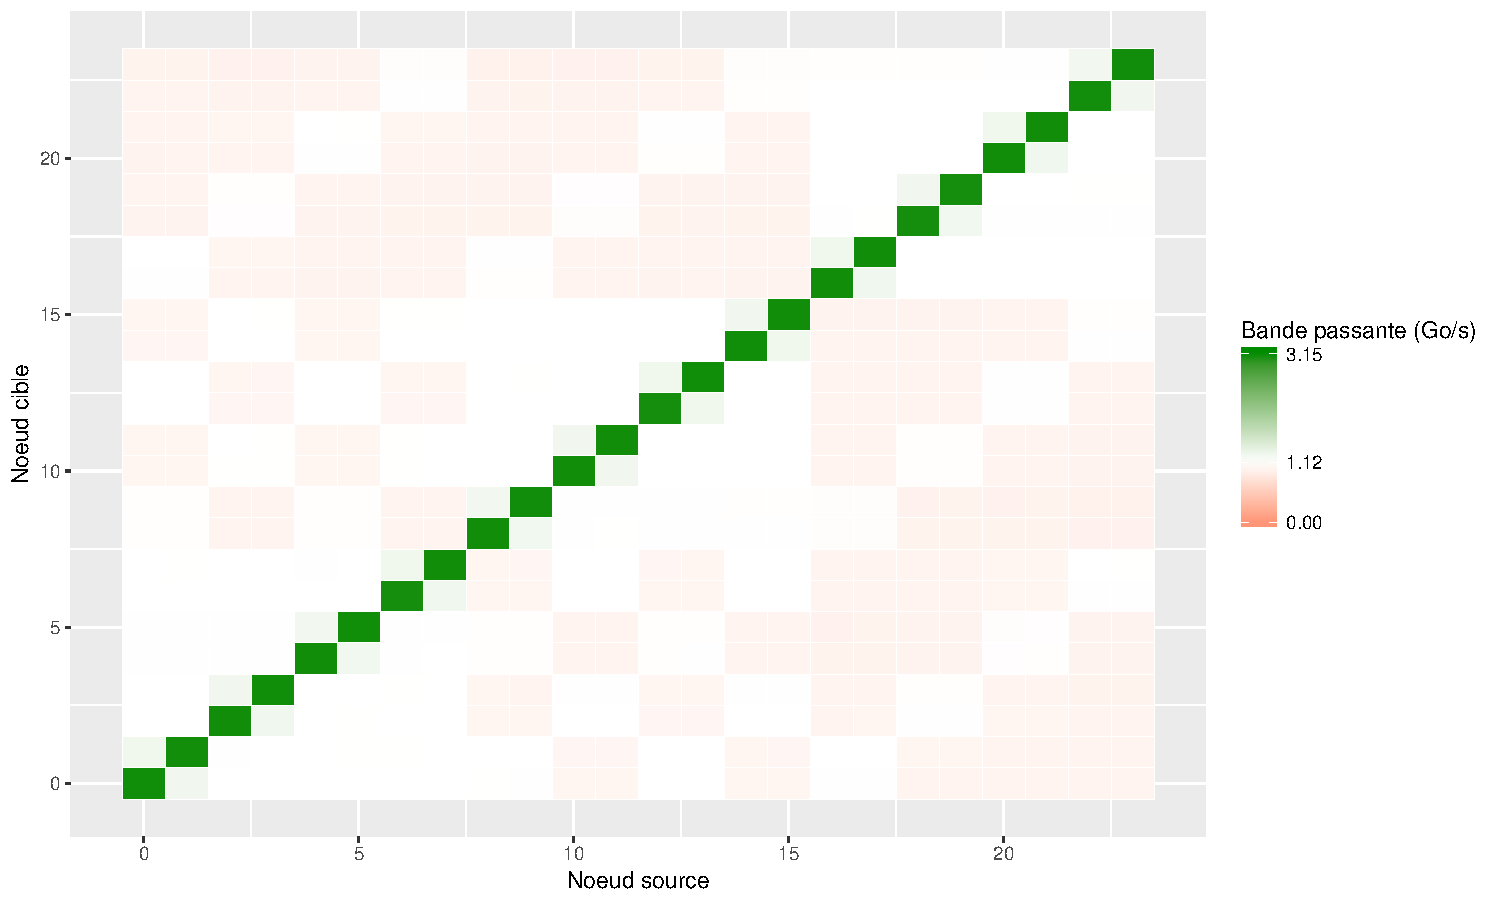
\includegraphics[width=\textwidth]{heatmap_idchire_memcpy}
  \caption{Carte de la bande passante d'idchire}\label{fig:contribs:machines:idchire:heatmap}
\end{figure}

\begin{figure}[h!]
  \centering
  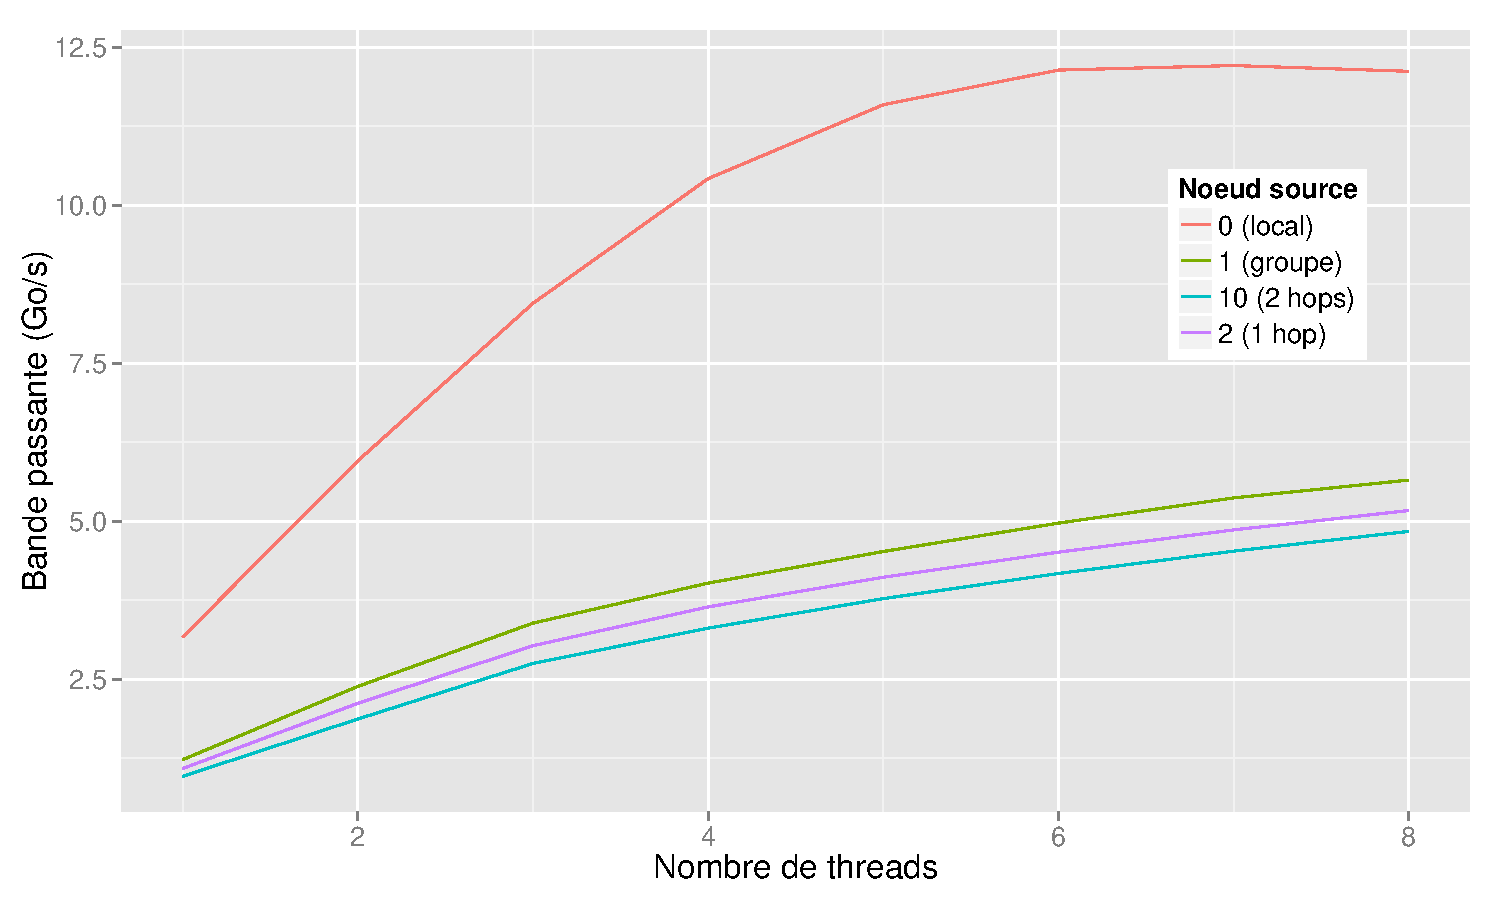
\includegraphics[width=0.9\textwidth]{link_saturation}
  \caption{Bande passante cumulée vers le nœud 0, en fonction du nombre de threads effectuant une copie et du nœud source}\label{fig:contribs:machines:idchire:saturation}
\end{figure}


La Figure~\ref{fig:contribs:machines:idchire:heatmap} présente la bande passante nœud à nœud en fonction de la source et de la destination, mesurée à l'aide d'une copie de tableau (|memcpy|) de 200 Mo.
Elle fait apparaître clairement une diagonale où la bande passante est significativement plus grande, illustrant le coût d'un accès mémoire local comparé à un accès distant.

Néanmoins cette simple <<carte>> ne suffit pas à caractériser complètement les temps d'accès aux nœuds NUMA, puisque qu'une seule communication ne va pas saturer la bande passante totale disponible, ni même illustrer l'impact de la contention.


\subsubsection{Mesure des liens}\label{sec:contribs:machines:idchire:liens}

En dehors de l'accès aux caches locaux, il y a 4 liens à quantifier, identifiés sur la Figure~\ref{fig:contribs:machines:idchire:topo-liens}.
Afin de mesurer chacun des liens, nous avons défini des scénarios spécifiques que nous avons exécuté via \outil~: pour un nœud NUMA source donné (ici 0), nous avons alloué et initialisé deux tableaux de 200 Mo. Le premier sur le nœud source, et le second sur le nœud local. Nous avons ensuite effectué une copie du tableau source vers le tableau local (via |memcpy|) et mesuré le temps de l'opération.
Pour chaque type de nœud source (même nœud, distant sur le même groupe, distant via un rebond, distant via deux rebonds), nous avons effectués de une à huit copies simultanées.


La figure~\ref{fig:contribs:machines:idchire:saturation} regroupe les résultats de la bande passante point à point, en fonction de nombre de copies simultanées ayant lieu, et en fonction du nœud d'où provient les données.
On constate que la bande passante maximum du lien local atteint 12.2 Go/s, et qu'il commence à saturer lorsque plus de la moitié des cœurs sont utilisés.
Le lien groupe plafonne à 5.6 Go/s, le lien distant 1 plafonne à 5.1 Go/s, et le lien distant 2 à 4.8 Go/s.
On peut également noter que les communications point à point sont symétriques.

\begin{figure}[ht]
  \centering
  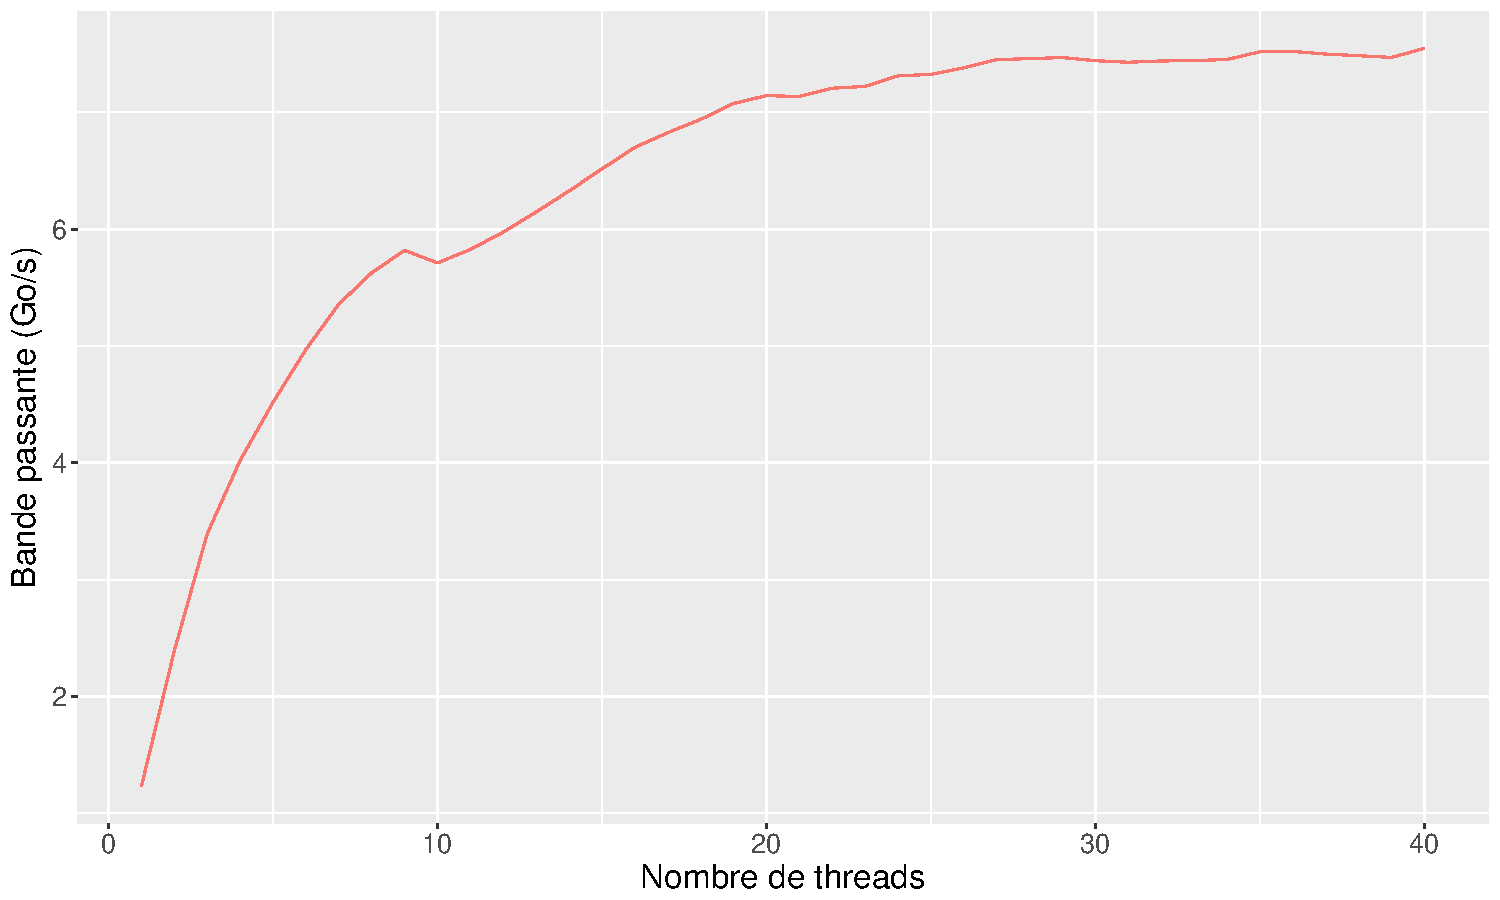
\includegraphics[width=0.9\textwidth]{link_output_saturation}
  \caption{Bande passante cumulée depuis le nœud 0 vers un nœud distant, en fonction du nombre de threads distant effectuant une copie}\label{fig:contribs:machines:idchire:saturation-output}
\end{figure}

Pour terminer la caractérisation de ces liens, nous avons finalement mesuré la bande passante maximale que l'on peut obtenir en <<sortie>> d'un nœud, en saturant les différents liens.
La figure~\ref{fig:contribs:machines:idchire:saturation-output} montre la bande passante cumulée lors d'une copie du nœud 0 vers un nœud distant, en fonction du nombre de threads effectuant une copie.
La bande passante maximale en sortie de nœud est donc de 7.5 Go/s, et commence à saturer aux alentours d'une vingtaine de copies distantes.

% TODO : si possible faire le lien saturation en sortie aussi, à voir si c'est pertinent de l'inclure


\subsection{brunch}\label{sec:contribs:machines:brunch}

Cette machine est équipée de 4 processeurs Intel(R) Xeon(R) CPU E7-8890 v4 (Broadwell), cadencés à 2.2 GHz.

Chacun de ce processeurs est associé à 378 Go de RAM pour former un nœud NUMA, ils disposent de 24 cœurs physiques partageant 60 Mo de cache L3 (20-ways associatifs).
Chacun des cœur à accès à 32 Ko de cache L1 (données) et 256 Ko de cache L2.
Les latences et bandes passantes relatives à chacun des niveaux de cache sont présentées dans le tableau~\ref{tab:synthese-processeurs}.

La machine entière dispose donc de 96 cœurs physiques, et de 1.5 To de RAM.
Les processeurs Broadwell disposent d'instructions FMA~\footnote{\emph{Fused Multiply-Add}, permettant d'effectuer une addition et une multiplication en une étape}, permettant d'effectuer 8 additions et multiplications de nombres flottant à double précision en un cycle, portant le pic de performance théorique de la machine à 3.3 TFLOPs.


\subsubsection{Topologie}

\begin{figure}[ht]
  \centering
  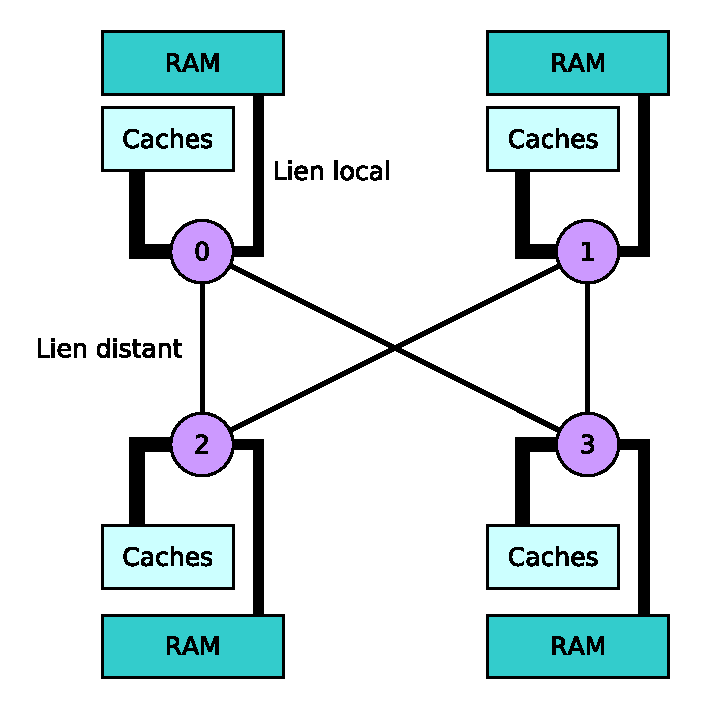
\includegraphics[width=0.6\textwidth]{topo-brunch}
  \caption{Topologie schématique complète de brunch}\label{fig:contribs:machines:brunch:topo-liens}
\end{figure}

L'interconnexion des nœuds NUMA est effectué à travers l'Intel \emph{Quick Path Interconnect} (QPI).
Contrairement à idchire, la topologie de la machine est relativement plate~: les nœuds sont directement connectés les uns aux autres, et seule la notion d'accès distant ou local permet de distinguer une hiérarchie.
La topologie complète de la machine est représentée sur la figure~\ref{fig:contribs:machines:brunch:topo-liens}

\begin{figure}[t!]
  \centering
  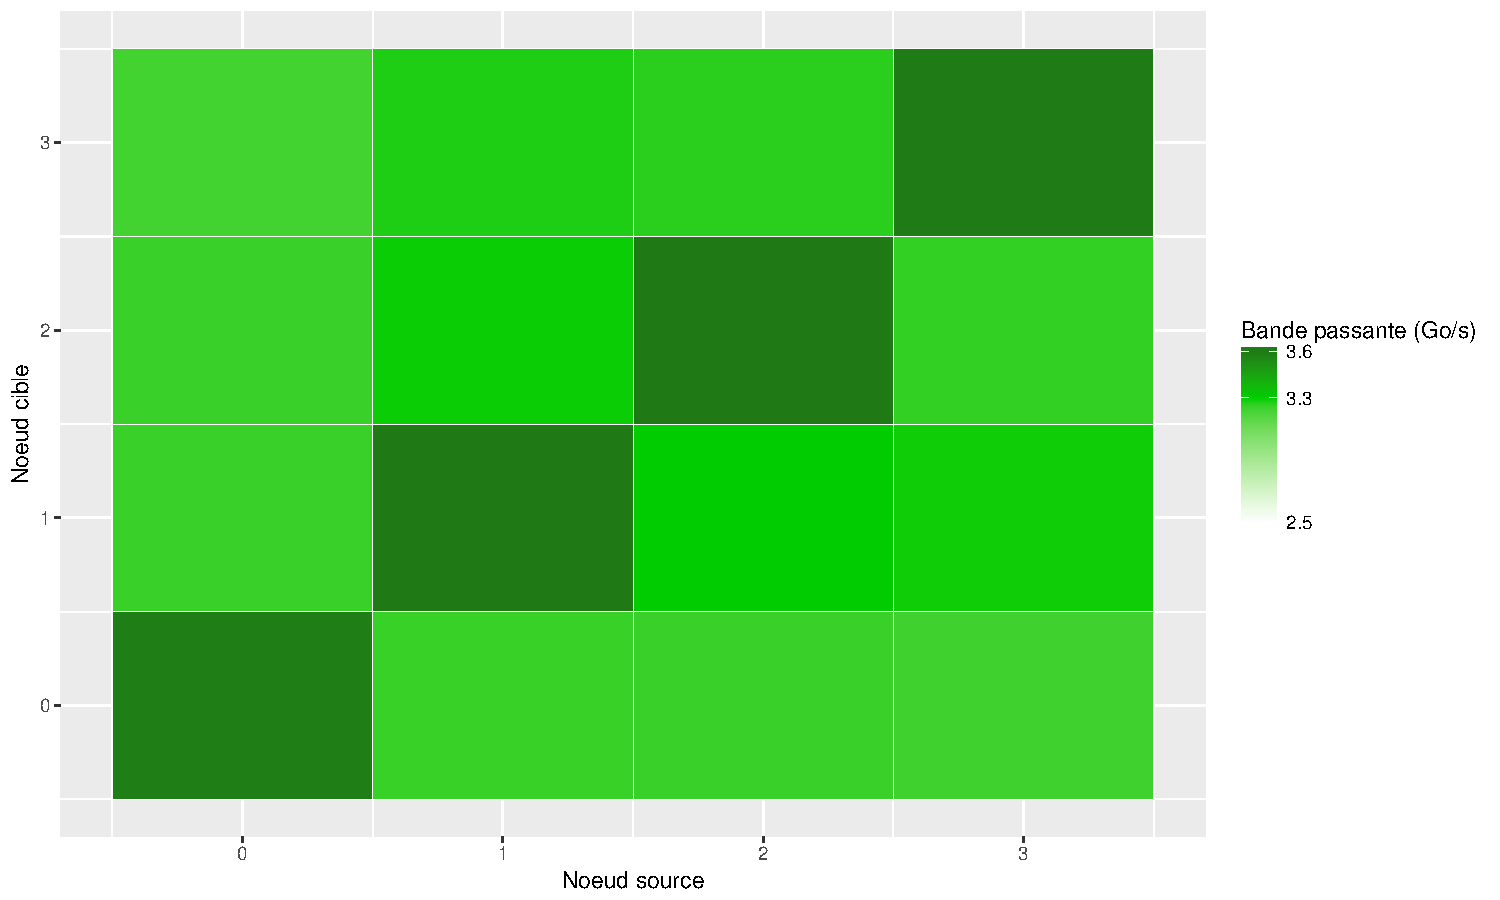
\includegraphics[width=\textwidth]{heatmap_brunch}
  \caption{Carte de la bande passante de brunch}\label{fig:contribs:machines:brunch:heatmap}
\end{figure}
\begin{figure}[h!]
  \centering
  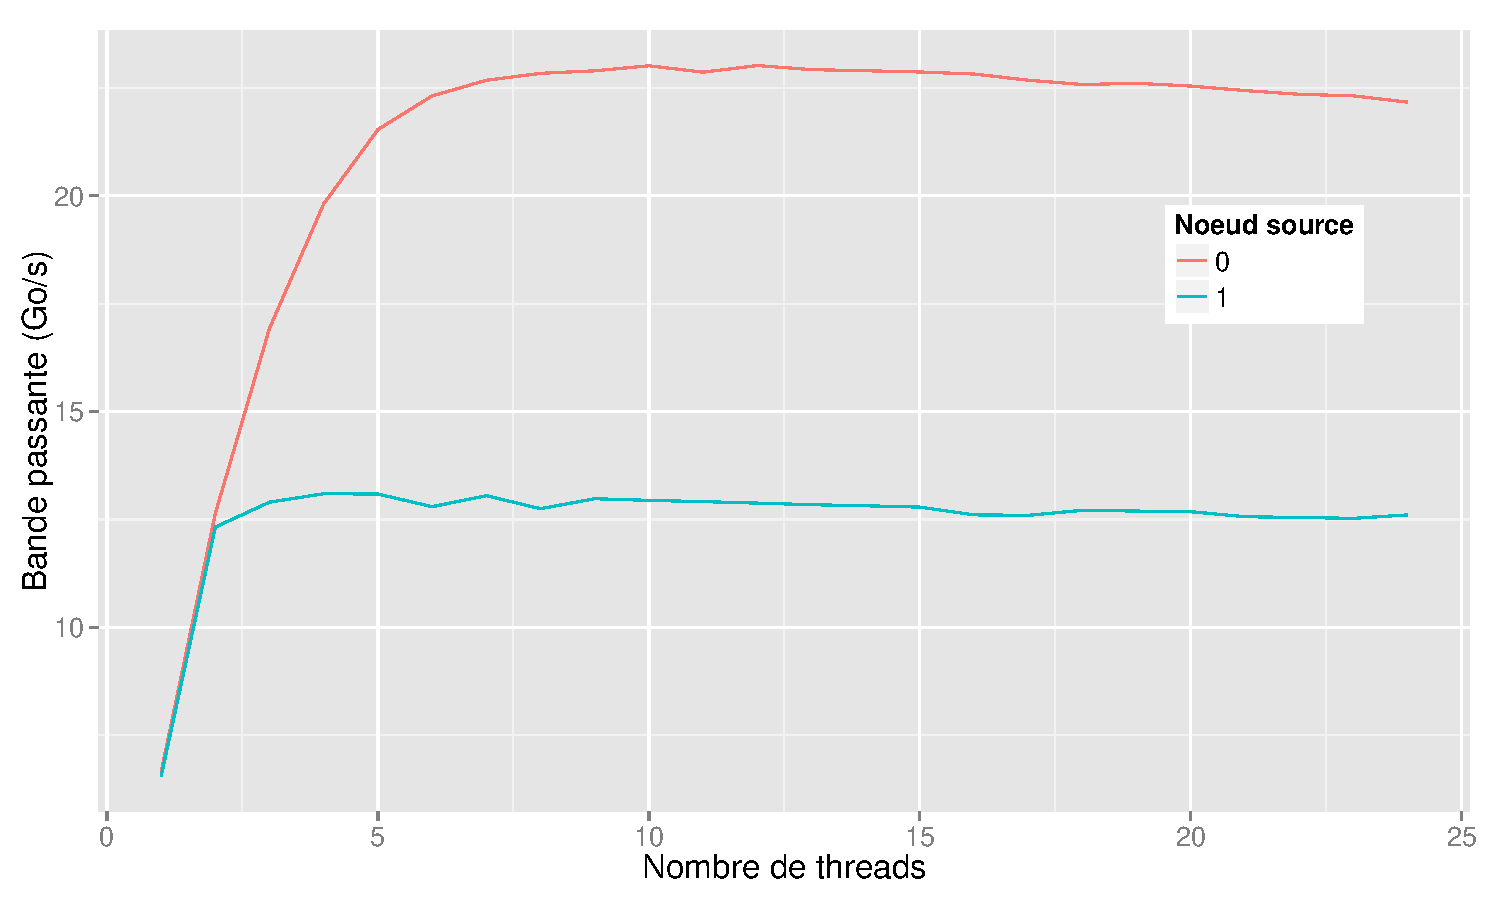
\includegraphics[width=\textwidth]{link_saturation_brunch}
  \caption{Bande passante cumulée depuis le nœud 0, en fonction du nombre de threads effectuant une copie et du nœud destination}\label{fig:contribs:machines:brunch:saturation}
\end{figure}


La Figure~\ref{fig:contribs:machines:brunch:heatmap} présente la bande passante nœud à nœud en fonction de la source et de la destination, mesurée à l'aide d'une copie de tableau (|memcpy|) de 200 Mo.
Bien qu'une diagonale se dégage clairement, la différence entre accès local et accès distant n'est de l'ordre que de 10\%, comme en témoigne l'échelle de couleur sur la figure.

\subsubsection{Mesure des liens}

De même que pour idchire, nous avons effectué des observations complémentaires pour caractériser plus précisément les liens locaux et distant, afin de déterminer leur saturation.
Les résultats de ces expériences ont été rassemblés sur la figure~\ref{fig:contribs:machines:brunch:saturation}.
Bien que la bande passante soit bien plus importante que sur idchire, les liens arrivent à saturation bien plus vite~: à peine 20\% de charge du nœud permet de saturer la bande passante.

\bigskip
\bigskip

Ces résultats sur les capacités physique des machines vont avoir un impact important dans la section suivante~: nous allons faire une étude de cas d'une application - la factorisation de Cholesky, et nous allons en étudier individuellement les parties critiques.
Certaines de ces parties critiques peuvent utiliser un large ensemble de données, en pleine charge de la machine les performances seront donc limitées par les résultats que nous venons de décrire.

